\chapter{Conclusion}
Herein we have constructed various different model mass-spring lattices on
which we have built up not just the mathematics, but also the codes, to allow
us to analyse the effects of different topological perturbations. This has led
us to discovering various different configurations of lattices which permit a
wide range of wave propagation manipulation. As we see that our results match
those obtained from other models, we anticipate that our model system is a good
approximation and can be used to model more complex waves. And from there, it
is our hope that this powerful ability to manipulate and channel wave energy as
we please can be used to further the good of humankind!

\bigskip
\bigskip

\begin{figure}[!h]
\centering
\begin{subfigure}[b]{.5\textwidth}
  \centering
  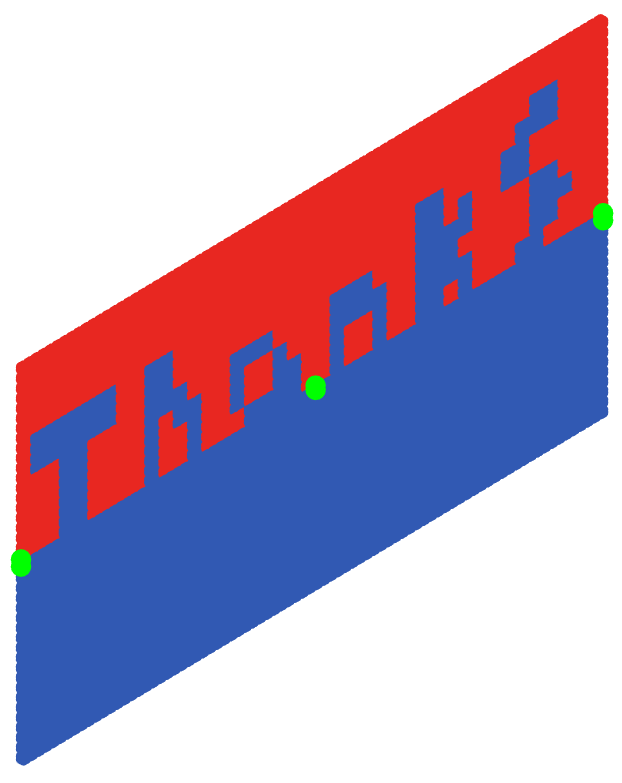
\includegraphics[width=0.7\linewidth]{imgs/thanksarr.png}
  \caption{Arrangement of cells.}
  \label{fig:sub1}
\end{subfigure}%
\begin{subfigure}[b]{.5\textwidth}
  \centering
  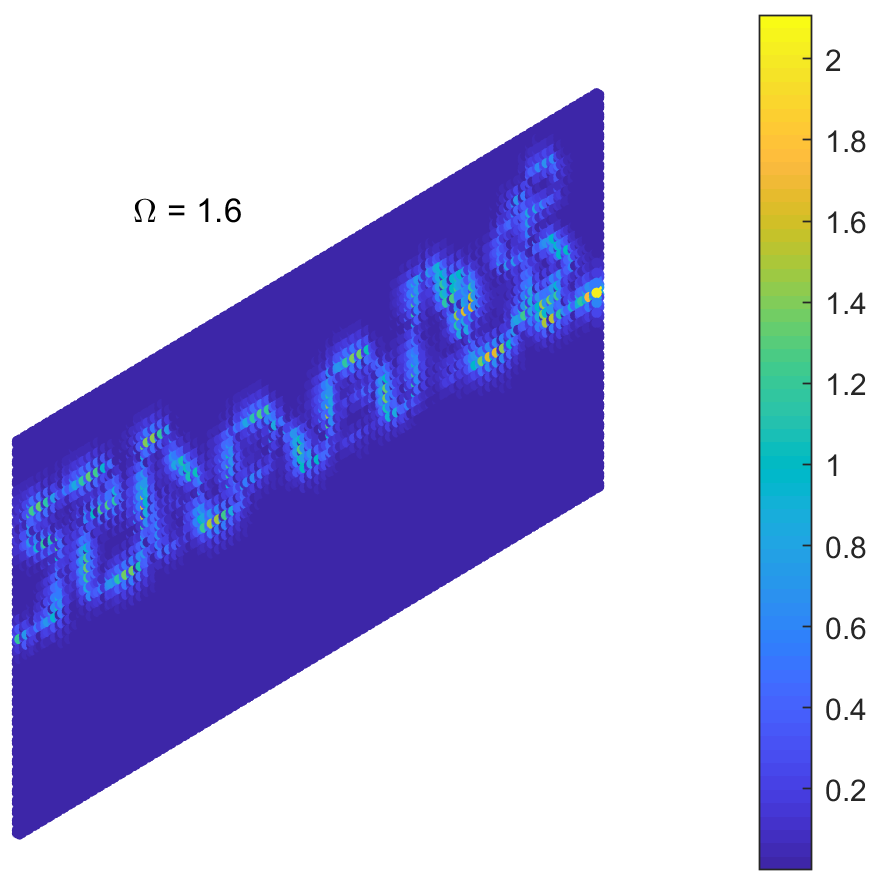
\includegraphics[width=1\linewidth]{imgs/thanksscat.png}
  \caption{The plot of $|y_i|$ for each mass in each cell.}
  \label{fig:sub2}
\end{subfigure}
\caption{Simulation of scattering on the hexagonal finite lattice with the
boundary spelling out a word commonly used in the English language to express
gratitude.}
\label{fig:thanks}
\end{figure}
